\documentclass[a4paper,12pt]{article}

\usepackage{url}
\usepackage{epsfig}
\usepackage{graphics}
\usepackage{fancyhdr}
\usepackage[parfill]{parskip} % Activate to begin paragraphs with an empty line rather than an indent
\usepackage{amsmath}
\usepackage{natbib}
\usepackage{subfigure}
\usepackage{svg}
\usepackage[T1]{fontenc}
\usepackage[utf8]{inputenc}
\usepackage{amsmath,amssymb}
\usepackage[russian,english]{babel}
\graphicspath{{pictures/}}

% SVG Options
\setsvg{inkscape = inkscape -z -D}
\setsvg{svgpath = pictures/}

\title{Carl Bildt Tweets: A comparison of regular and constrained Markov chain for text generation}
\author{\hspace*{-0.5cm}
Group Ain't intelligent\\
\begin{tabular}{cccc}
Viktor Bj\"{o}rkholm & Jesper Br\"{a}nn & Daniel Duberg & Jakob Tidestr\"{o}m\\
92-11-17 & 92-09-30 & 93-01-17 & 90-10-04 \\
viktorbj@kth.se & jbrann@kth.se & dduberg@kth.se & jakobti@kth.se \\
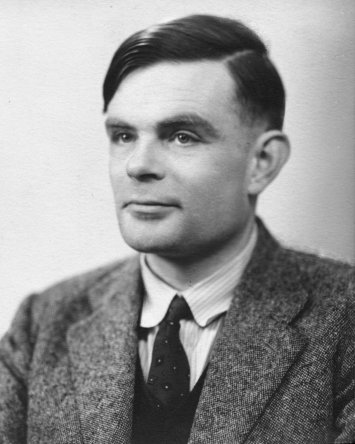
\includegraphics[width=0.13\linewidth]{Alan_Turing_photo} & 
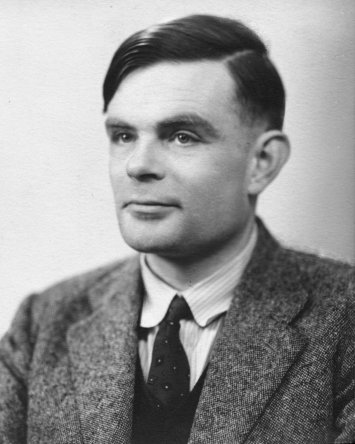
\includegraphics[width=0.13\linewidth]{Alan_Turing_photo} & 
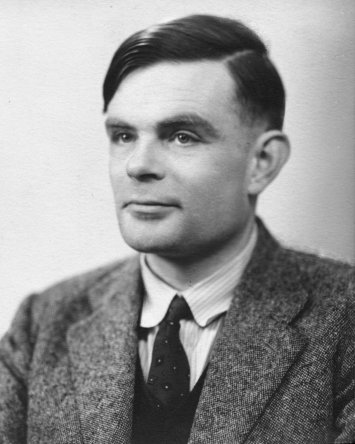
\includegraphics[width=0.13\linewidth]{Alan_Turing_photo} & 
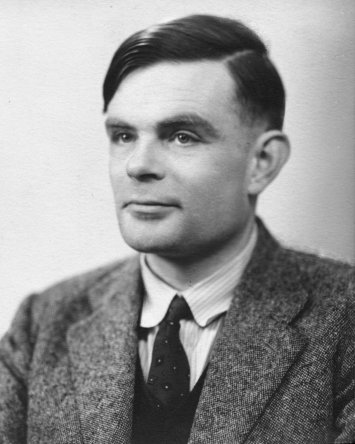
\includegraphics[width=0.13\linewidth]{Alan_Turing_photo}
\end{tabular}} 
% Normally there will not be any pictures but we want
% these so that we can connect faces to names in the course
% We also want birthdates so that we can tell people with the same
% name apart
\date{}

\pagestyle{fancy}
\setlength{\headheight}{15pt}
\fancyhf{}
\lhead{DD2380 ai14} % DO NOT REMOVE!!!!
\rhead{V. Bj\"{o}rkholm, J. Br\"{a}nn, D. Duberg, J. Tidestr\"{o}m} %% UPDATE WITH YOUR NAMES

\begin{document}

\maketitle
\thispagestyle{fancy}

\begin{abstract}
This paper explores the difference in result when generating twitter messages that seem to come from a former Swedish foreign minister, Carl Bildt, using two natural language generation based techniques that build on each other.
The outcome of the methods were indeed tweets seeming to originate from Carl Bildt with a subject that circulated around foreign politics. 
The most reliable ones however were mainly copied directly from his feed; this problem is addressed using the methods discussed in this paper. The methods used in this paper are Markov chains with and without constraints to generate tweets, suggestions are also given on improvement of our technique.


\end{abstract}



\clearpage

%%%%%%%%%%%%%%%%%%%%%%%%%%%%%%%%%%%%%%%%%%%%%%%%%%%%%%%%%%%%%
%%%%%%%%%%%%%%%%%%%%%%%%%%%%%%%%%%%%%%%%%%%%%%%%%%%%%%%%%%%%%
\section{Introduction (1--2 pages)}
\label{sec:intro}
% What is the problem and why is it important? 
% What will the reader get out of it? 
% Present specific results
% Dont go into detail 
This paper aims to develop an understanding on refining natural language text generation.
Natural Language Generation (NLG) is an area of research within the field of Artificial Intelligence. 
The purpose of NLG is to generate text that is semantically correct in order to make communication with computer systems more natural and understandable for users.

Within this paper we show the difference in quality of two different approaches to text generation. 
One of these approaches is using Markov chains or more commonly known as n-grams. 
These n-grams take n words in sequence and uses a corpus of text to guess what the most probable next word is. 
Using a larger n in an n-gram means that more text is copied straight from the corpus, 
however this also means that there is a higher likelihood that the text being generated is meaningful. 
% Givet att corpus är meningsfullt
We will contrast this method with using constrained Markov chains. 
The main constraint of the Markov chains is that two words following each other will have the same sequence of part-of-speech as the corpus.
Part-of-speech is a concept within NLG that divides a text into the different linguistical categories of the words within it.

We aim to show that using this constraint upon the Markov chain, sentences will have a greater diversity but still be as semantically correct as just using a n-gram.
Since the problem with larger n:s within n-grams is that text is copied straight from the corpus, 
the constraint will hopefully help us create semantically correct sentences with a greater diversity from the corpus.

To be able to show differences in these two approaches we generate Twitter messages, so called tweets. 
We build upon the work by \cite{shannon48} for the theory of implementing an n-gram, a description on generating and parsing corpuses by \citep{Corpus}
and the work by \citealp{McBarb} to implement our own constraints on the n-gram.
   
\subsection{Contribution}
% Förklara för en datalog varför det vi gjort ar vettigt.

We have implemented a unigram of part-of-speech (POS) on to a bigram in order to observe the difference in the result. 
As mentioned above a problem with n-grams with to high n:s is that they will simply copy parts of the corpus if said corpus does not contain a large variation of similar sentences, 
so that a given start of n words does not automatically lead to one sentence finish. i.e. a larger corpus is needed for larger n:s.
To be able to keep a smaller and diverse corpus we applied the unigram of POS tags on top of the n-gram to allow the program to select words of a common word type order and with a greater diversity than naturally occurs in the corpus.

Our main contribution to the field is that we have tried putting this unigram constraint upon the regular Markov chain and doing it for short message generation.
The research area we base this paper on focus on generating text that fits a theme or rhythm whereas we generalize the concept by creating text that is not constrained by a pre-written sequence of POS. 
Our approach is that we let the model be trained with two types of information, thus our contribution to the field lies in examining how the combination of these two approaches improves the general natural language generation.


%A lot new research involves the constraining of Markov chains to produce text that fits different molds than just text generated from a corpus. 
%It is important to be able to generate text that is 

\subsection{Outline}
We bring up the relation of our work to some other work in the field. We explain how \citep{shannon48}, \citep{Corpus} and \cite{McBarb}'in section~\ref{sec:relwork} and explain how that research has affected ours. 
In section~\ref{sec:method} we then go through the details on how the algorithm works, 
we also give examples to explain in detail what the difference between the two methods we are comparing. 
This is complemented with details regarding our specific implementation of the algorithm in section~\ref{sec:impl}. 
The data from running the algorithm is explained, reviewed and evaluated in section~\ref{sec:exps}.

%%%%%%%%%%%%%%%%%%%%%%%%%%%%%%%%%%%%%%%%%%%%%%%%%%%%%%%%%%%%%
%%%%%%%%%%%%%%%%%%%%%%%%%%%%%%%%%%%%%%%%%%%%%%%%%%%%%%%%%%%%%
\section{Related work (1--3 pages)}
\label{sec:relwork}
% It is here we show that we know the field well and present the reports that we have read
%% Saker vi behöver svara på i detta stycke:
% Vad vet vi om hur dem använde constraints i sitt arbete? Vi verkar ju inte veta något om det eftersom vi bara gissar oss fram :D
%
% Har vi något mer att basera vårat arbete på? En vetenskaplig text är ju bra, men om vi läst fler så är ju det rätt bra.

% Jesper skriv under härate sentenses from words.
In \cite{shannon48} Shannon goes through the first basic steps in how to naively generate text from a corpus with Markov chains. 
He explains in depth how Markov chains can be used to generate real sounding English words from letters and also sentences from words. 
We implemented n-grams and tried different orders of them which according to Shannon would generate output more similar to the content of the corpus with the higher orders. 
The difference between the different orders of Markov chains lies in how many preceding states that are taken in consideration.
Our Markov chain was built up with a transition matrix where the values of the rows in a column represent the probability of moving from the state of the column to the state of the row. The probabilities of the transitions between the different states is taught to the transition matrix by iterating through the corpus. This concept is introduced by Shannon and proven to work in his paper.
His approach was novel at the time however it is a staple in modern text generation. 


% Nisse skriv under här % Nisse-nisseus
In the in-proceedings by \cite{Corpus}, they describe the process of building a corpus for a natural language generation system with different user requests and demands that constrain the corpus. 
The corpus consists of example output that the NLG will imitate and the user requests should be applied through modifying and simplifying the corpus according to them.
Since the corpus should consist of example output, and we want to generate text that should imitate tweets, we populate our corpus with tweets.
As we play the role of our own users since we are the ones with demands on the generated text and we need to generate a corpus that is usable by our algorithms. Thus, as \citep{Corpus} describe we remove things from our corpus that we do not want to use when generating, such as hash-tags and URLs.


Our work on actually constraining the Markov chain is built upon \cite{McBarb} work, 
where the authors generated lyrics from different artists using Markov chains with constraints. 
These were to be generated in a specific style and with a rhythm, to simulate real lyrics from a large span of artists, which is achieved by applying constraints on a bigram, a Markov chain of order 2.
They use POS templates to fit the correct poetic metre, these templates are not generated by their algorithm, but rather handcrafted to get a proper result.
Our take from this paper was to be able to apply constraints upon a bigram, or rather a Markov chain in general. Similarily we utilize a part-of-speech template of sorts, but we diverge a bit from this paper by not handcrafting them and instead letting our algorithm generate them based on the corpus.


%%%%%%%%%%%%%%%%%%%%%%%%%%%%%%%%%%%%%%%%%%%%%%%%%%%%%%%%%%%%%
%%%%%%%%%%%%%%%%%%%%%%%%%%%%%%%%%%%%%%%%%%%%%%%%%%%%%%%%%%%%%
\section{My method (1--4 pages)}
\label{sec:method}
Our method that forms the basis of this paper is generating Twitter messages with the use of both Markov chains and constrained Markov chains and to compare the two methods with each other.
The theory is that constraining an Markov chain will yield better and more diverse text being generated. 
In section~\ref{sec:exps} where we explain our experiments and data we try out a different order of the Markov chain, 
for the sake of explanation we assume a first order Markov chain is used to explain how the method works. 
In a limited corpus such as this one: \\

\begin{tabular}{r | l}
``Rolf has a dog.`` & Noun $\to$ verb $\to$ singular quantifier $\to$ noun \\
``Rolf owns a dog.`` & Noun $\to$ verb $\to$ singular quantifier $\to$ noun \\
``Rolf can not walk his dog.`` & Noun $\to$ modal $\to$ adverb $\to$ verb $\to$ pronoun $\to$ noun \\
\end{tabular}

This corpus generates a Markov chain that looks like figure 1a, with the edges being the probabilities for the specific transitions. 
In the figure the specific part-of-speech is included in the states beneath the words from the corpus. 
If we then add constraints from a transition matrix, built up from POS-analysis of the same corpus we are given the new chain that is seen in figure 1b.

\begin{figure}[h!]
  \hfill
  \subfigure[Unigram of the limited corpus]{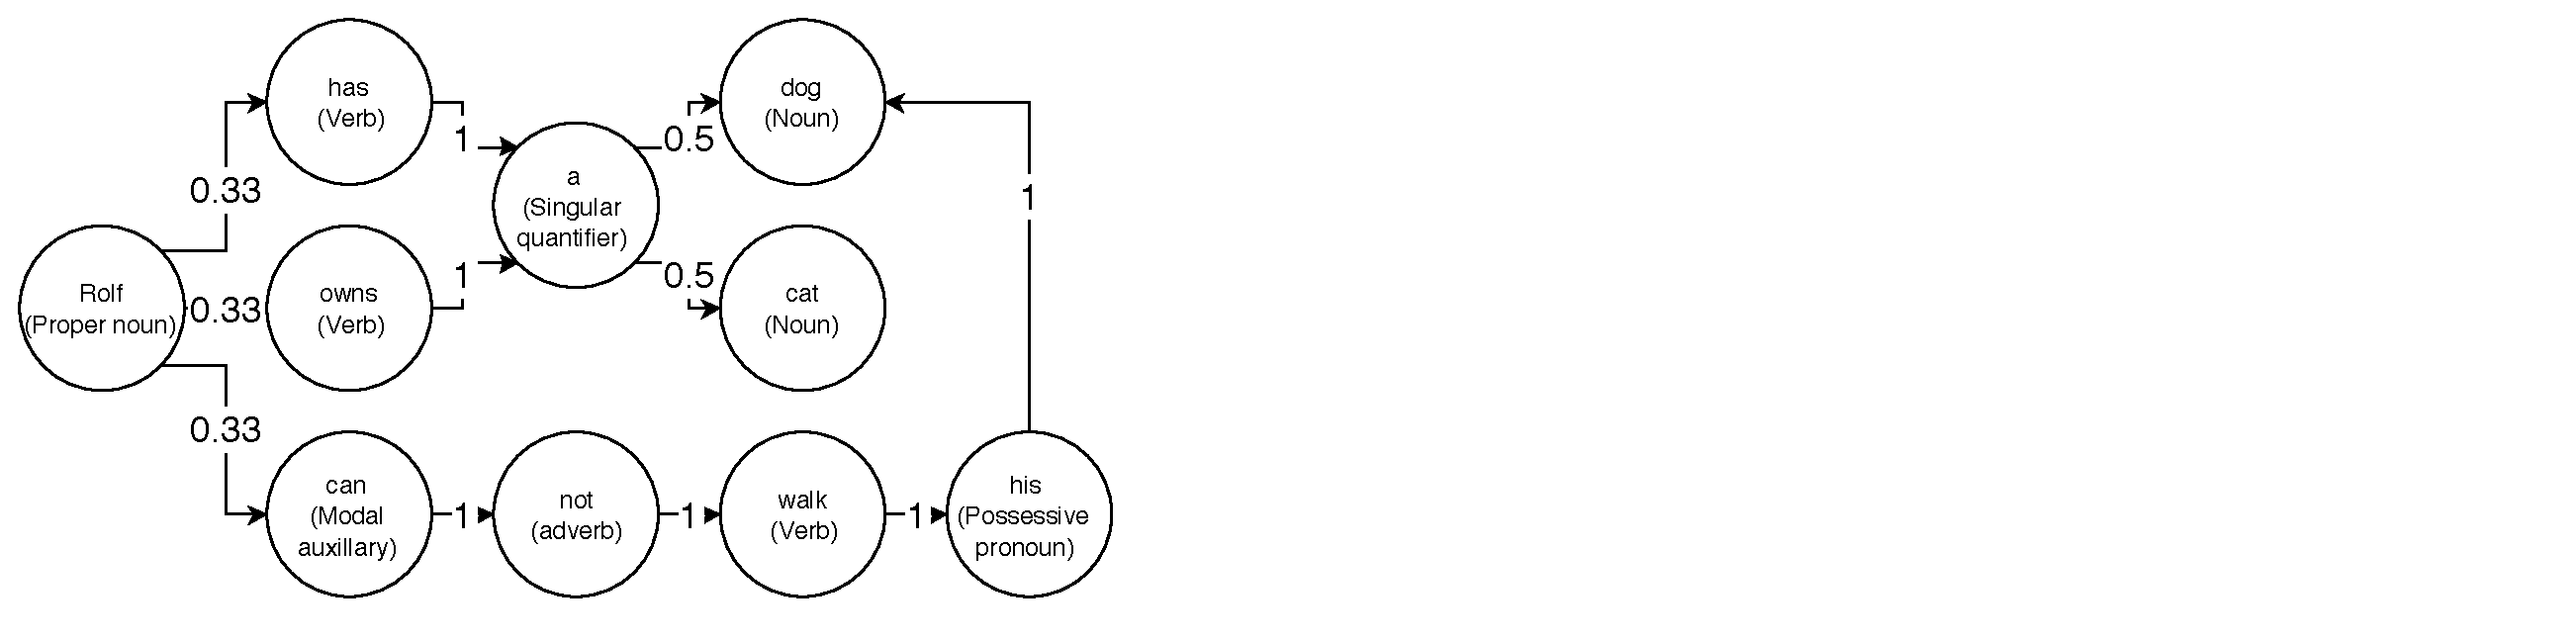
\includegraphics[width=0.49\linewidth]{Bigram1.pdf}}
  \hfill
  \subfigure[Unigram with constraints applied]{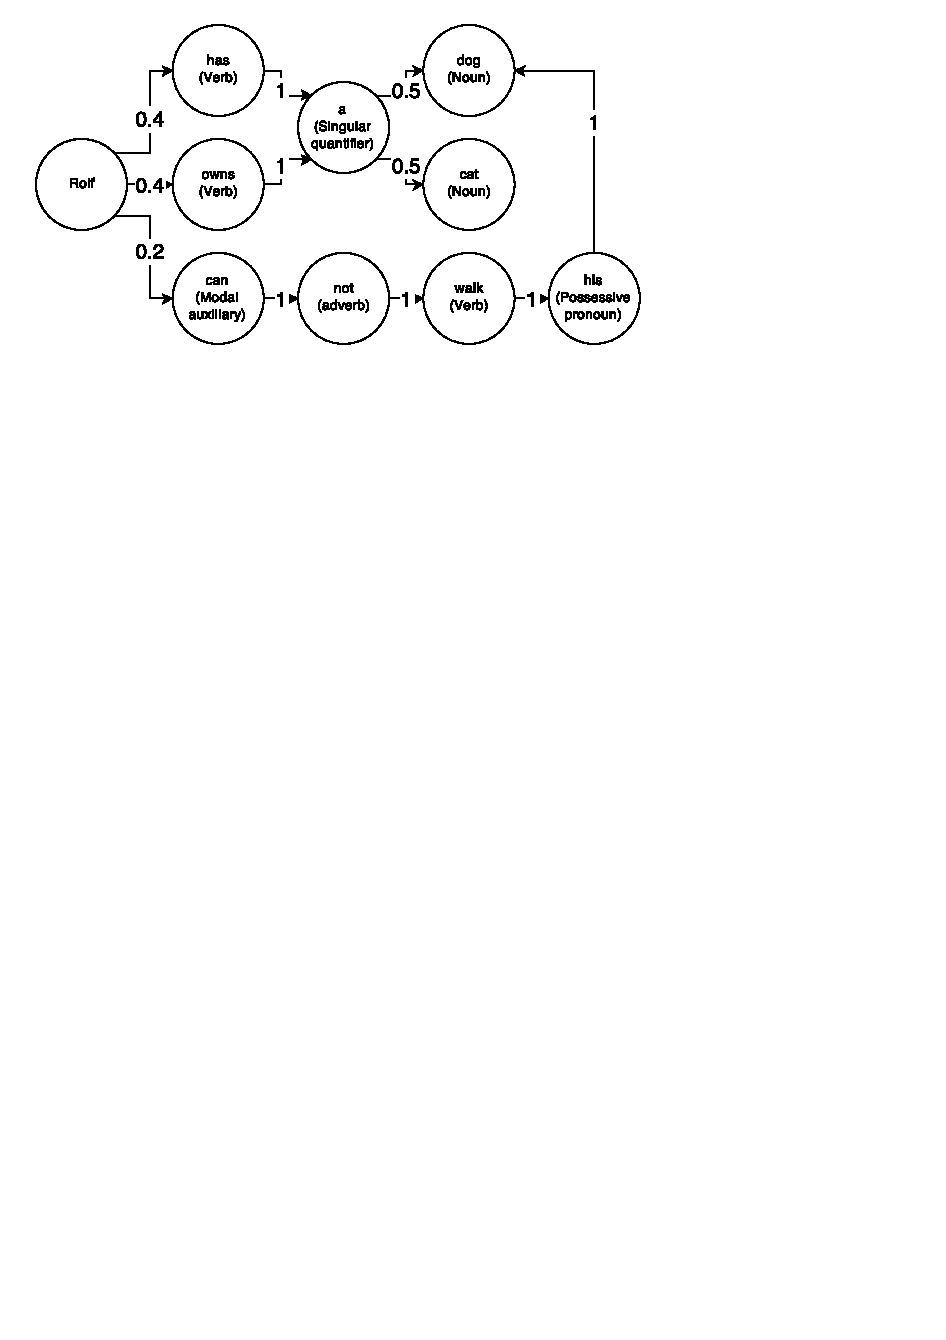
\includegraphics[width=0.49\linewidth]{Bigram2.pdf}}
  \hfill
  \caption{Unigrams}
 \end{figure}



We can see in figure 1b that since both ''has`` and ''owns`` are verbs they are more probable to occur than ''can``, this is reflected in the new edges. 
This happens because the part-of-speech ''verb`` is more likely to follow a personal noun according to our transition matrix, and thus ''has`` and ''owns``, who are 
both verbs become even more likely to follow a personal noun. This method can then be further applied to a bigram, a trigram or any n-grams that follows. 
Our method however will only have an unigram for the transition matrix, even if the Markov chain of words from the corpus is longer, 
the transitions are only observed with one previous state in consideration.

\subsubsection{Calculating uniqueness}
We originally wanted to analyse the semantic correctness of our tweets but were unable to find a method of doing so mechanically. In lieu of other options we decided to instead analyse how unique the tweets were in terms of how much it just copied straight out of the corpus.

Since we use a bigram it will always take three successive words but anything above that compromises uniqueness.

For example purposes we added these sentences to the limited corpus mentioned earlier:

\begin{tabular}{l}
``Mufasa is a dog with a purple tail.``\\
``Mufasa owns a yellow cat.``\\
``Jessica can not eat a yellow dog with a pink tail.``\\
``Steve has a shirt with a purple tail.``\\
\end{tabular}

% Räkna manuellt med limited corpus
\textbf{Example 1:} ``Rolf can not eat a yellow cat.``
	
It first matches "can not eat a yellow" since it is the largest continuous match. This match contains five words, which is two words longer than it has to be (since we use a bigram), this reduces uniqueness by 2. What is left is the strings "Rolf" and "cat", since each of these strings are shorter than three words we stop here.

Thus this sentences uniqueness is $\frac{7 - 2}{7} \approx$ 71 percent.

\textbf{Example 2:} ``Rolf has a shirt with a yellow dog with a pink tail.``
	
The first match is "a yellow dog with a pink tail", reducing uniqueness by 4. Remaining is "Rolf has a shirt with" which matches "has a shirt with", further reducing uniqueness by 1. Only "Rolf" is left over thus we stop. 

Thus this sentence has a uniqueness of $\frac{12 - (4 + 1)}{12} \approx$ 58\%.

\subsubsection{Corpus}
In order to generate tweets, we first discussed the problem regarding the semantical corectness of a generalized tweet.
The average level is according to our own experience far from sematically correct, which isn't a problem in understadabillity for an experienced Twitter user,
but is a problem for our POS who would not recognize the words. Even if it would give it an ''unknown``-tag, we would not be able to predict any kind of results.

\begin{figure}[h!]
  \centering
  
\includegraphics[width=0.75\linewidth]{machine_learning}
  \caption{An example tweet}
\end{figure}

To solve this problem approximatily, we decided to generate tweets for a specific user who mostly uses correct grammar and semantics when tweeting and tweets in English.
Our option fell on Carl Bildt, former foreign minister of Sweden, because of his active use of Twitter, 
that he tweets in English and that most of his tweets are in grammatically correct English.

\subsection{Implementation (0--2 pages)}
\label{sec:impl}
The implementation relied on a Part-of-Speech tagger from Stanford's Natural Language Processsing group.

We start by collecting data, in the form of tweets, by a target person, Carl Bildt, to be used as the corpus of our tweet generator. The data is filtered to remove unwanted elements such as hashtags and web addresses.

Each tweet is run through Stanford's speech tagger to get the lexical class of each word depending on context.
We then use these lexical classes as states for the transition matrix, more specifically they're used to see what lexical class usually follows any given lexical class or terminates a sentence.

While iterating through the gathered data we store what word follows any given two words, including sentence terminating symbols such as '.' or '!' and store it as a bigram.

When generating tweets two methods are used, first the bigram gets to select which words to use entirely on its own digression (Markov chain). Then the process is repeated but this time the bigram is constrained by which lexical class of words it is allowed to choose from, that class being whichever one the transition matrix has decided should follow (constrained Markov chain).

%%%%%%%%%%%%%%%%%%%%%%%%%%%%%%%%%%%%%%%%%%%%%%%%%%%%%%%%%%%%%
%%%%%%%%%%%%%%%%%%%%%%%%%%%%%%%%%%%%%%%%%%%%%%%%%%%%%%%%%%%%%
\section{Experimental results (1--4 pages)}
\label{sec:exps}

\subsection{Experimental setup}
We generate 10000 tweets with a length of between 30 and 140 characters using both the Markov chain and the constrained Markov chain.

Once generated we analyse the tweets uniqueness by counting how many of the used words are from the same part of the corpus. However, since we use a bigram three of the words have to appear in succession and thus we only count if four or more of the words are from the same part of the corpus. We then divide this by the number of words to get an average for the whole tweet.

\newpage
\subsection{Experiment}

\subsubsection{Uniqueness based on words in tweet}

\begin{figure}[h!]
  \hfill
  \begin{center}
  	{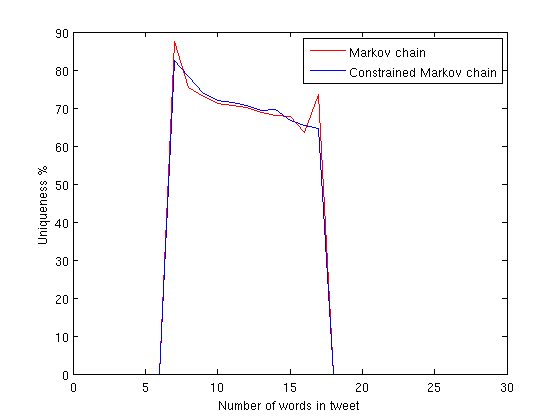
\includegraphics[width=300, height = 140]{UniqByNumWordsTweet.png}}
  \end{center}
  \caption{Uniqueness based on words in tweet}
 \end{figure}
 
 Uniqueness drops as the number of words in the tweet increases, both Markov chain and the constrained Markov chain decrease at  approximatively the same rate however. This is because of how our algorithm for uniqueness works, namely that if the tweet has 6 words then at worst it can take all 6 words from the same part of the corpus. This will result in a uniqueness of 50 percent, since this is a worst case scenario it cannot be lower that this.
 
 \begin{figure}[h!]
   \hfill
   \begin{center}
  	{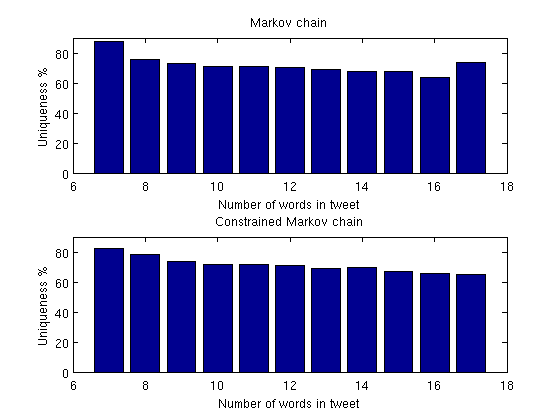
\includegraphics[width=280, height = 140]{UniqByNumWordsTweet2.png}}
  \end{center}
  \hfill
  \caption{Uniqueness based on words in tweet (Comparison)}
 \end{figure}
 
 On average the constrained Markov Chain produces tweets that are 71.04 percent unique and the Markov Chain has an average uniqueness of 70.29 percent. This means the constrained Markov chain constructs, on average, tweets that are 1.01 percent more unique.

\newpage
\subsubsection{Number of tweets based on uniqueness}

\begin{figure}[h!]
  \hfill
  {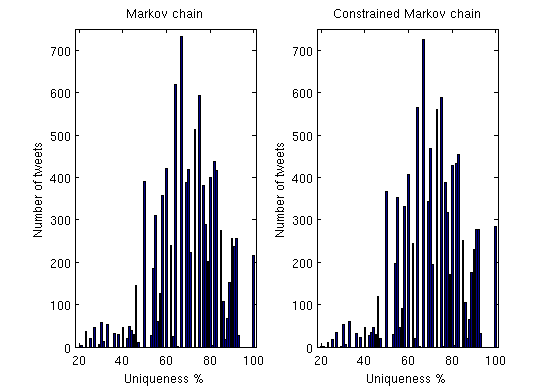
\includegraphics[width=1\linewidth, height = 165]{NumTweetsByUniq.png}}
  \caption{Number of tweets based on uniqueness}
 \end{figure}
 
 Here too both the Markov chain and the constrained Markov chain have similar results as a whole but the Markov chain has more tweets with less uniqueness than the constrained Markov chain. The opposite is also true, the constrained Markov chain has more tweets with more uniqueness than the Markov chain.
 
  \begin{figure}[h!]
   \hfill
  {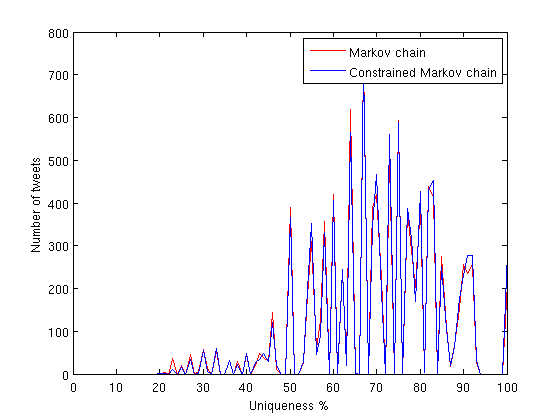
\includegraphics[width=1\linewidth, height = 165]{NumTweetsByUniq2.png}}
  \hfill
  \caption{Number of tweets based on uniqueness (Comparison)}
 \end{figure}

Figure 6 makes this more obvious, if you look at the lower end the Markov chain has visible spikes on the lower end (namely around 23 and 46 percent) and the constrained Markov chain has the same on the higher end (70, 82, 91 and 100 percent).

\subsubsection{Actual content of tweet}
Even though we could not mechanically analyse semantic correctness of our tweets we still looked at some of the tweets it generates. We generated 5 example tweets, using both methods, for analysis.

\textbf{Markov chain}

\begin{tabular}{l}
``Of risk of situation in Ukraine. By Pyongyang standards.``\\
``Victory Day has a great time!\hspace{0 cm}``\\
``And clear messages from Brussels after two days. The final rally of the.``\\
``Third capital today. Symbolic that US wins over Russia.``\\
``Well, Cold War it was? For a day in the clowns''.``
\end{tabular}

\textbf{Constrained Markov chain}

\begin{tabular}{l}
``\selectlanguage{russian}Очевидно обострение экономической войны Russia is good.``\\
``Truly alarming development in Bosnia.``\\ % INTE helt kopierad
``Started the meeting in Brussels. Istanbul after a couple of grey suits as well.``\\
``We have every reason to follow the different parts of Eastern Ukraine.``\\
``PM's Reinfeldt of Sweden. Most of our world. Looks worse than a dog.``
\end{tabular}

Occasionally the beginning and end of our generated tweets are semantically incorrect, this is caused by our corpus filtering as the preceding/subsequent element has been removed from the corpus.

We do not filter languages so sometimes we get long strings of, for example, Russian that we cannot determine if they are semantically correct or not.

Otherwise the subjects of the generated tweets all seem to revolve around politics and foreign relations and could therefore possibly be from a foreign minister.

Regardless of the method used to generate them the tweets are similar.

\newpage
%%%%%%%%%%%%%%%%%%%%%%%%%%%%%%%%%%%%%%%%%%%%%%%%%%%%%%%%%%%%%
%%%%%%%%%%%%%%%%%%%%%%%%%%%%%%%%%%%%%%%%%%%%%%%%%%%%%%%%%%%%%
\section{Summary and Conclusions (0.5--1 page)}
\label{sec:summary}
% Vad har vi kommit fram till?
We compared generating natural language with a native bigram from our corpus with using a constrained Markov chain of order 2 to generate tweets seeming to origin from a specific person, which in our experiment was Carl Bildt. 
The tweets should thus be semantically correct and have a somewhat meaningful content.
In the result we can see that using a constrained Markov chain has a slight advantage over simply using a bigram in generating a diversity of content. 
However, there was seemingly no difference at all in the quality of the content. 
They did seem to be from Carl Bildt, since the topics of the tweets were affected by the words in his tweets. 
A lot of the generated tweets had a political theme where conflicts were discussed and political situations in different regions of the world. 


% Vad bidrog det med?
We were able to show that applying constraints on a bigram made little difference rather than just using a bigram. We show that our approach adds a lot of work with small gain, however the gain results in mostly nonsensical text. When the diversity in the generated tweet increased it made the quality of the tweet decrease.

% Hur kan våra resultat förbättras/förändras?
The constrained matrix only uses a unigram, if it would use a bigram for it's POS constraints, perhaps the outcome would have been different. The outcome would probably be affected by it, however it is hard to say whether it would improve the results a lot. If the Markov chain was constrained by another property than the sequence of POS in Carl's tweets the results could possibly be different. An alternative could be to generate a template with topics that divide the tweet into parts and let that be the constraint of the Markov chain instead.

\newpage
%%%%%%%%%%%%%%%%%%%%%%%%%%%%%%%%%%%%%%%%%%%%%%%%%%%%%%%%%%%%%
%%%%%%%%%%%%%%%%%%%%%%%%%%%%%%%%%%%%%%%%%%%%%%%%%%%%%%%%%%%%%
\bibliographystyle{plainnat}
\bibliography{reflist}


\end{document}
